\section{Root Finding and Minimization}

\subsection{Some Notation}
\begin{itemize}
    \item Given $f(x):\mathbb{R}^n\rightarrow\mathbb{R}$, $\frac{\partial f}{\partial x}\in\mathbb{R}^{1\times n}$ is a row vector. This is because $\frac{\partial f}{\partial x}$ is the linear operator mapping $\Delta x$ into $\Delta y$, considering the shape alignment:
    \begin{equation}
        f(x+\Delta x)\approx f(x)+\frac{\partial f}{\partial x}\Delta x
    \end{equation}
    \item Similarly, $g(x):\mathbb{R}^m\rightarrow\mathbb{R}^n$, $\frac{\partial g}{\partial x}\in\mathbb{R}^{n\times m}$ for the same reason.
    \item These conventions make the chain rule work:
    \begin{equation}
        f(g(x+\Delta x))\approx f(g(x))+\left.\frac{\partial f}{\partial x}\right|_{g(x)}\left.\frac{\partial g}{\partial x}\right|_x\Delta x
    \end{equation}
    \item For convenience, we will define:
    \begin{align}
        \nabla f(x)=\left(\frac{\partial f}{\partial x}\right)^T\in\mathbb{R}^{n\times1}, \text{column vector}\\
        \nabla^2 f(x)=\frac{\partial}{\partial x}\left(\nabla f(x)\right)=\frac{\partial^2 f}{\partial x^2}\in\mathbb{R}^{n\times n}
    \end{align}

    \item 在本课中，谈及梯度gradient时，总是认为因变量是一维的。如，我们有拉格朗日函数$L(x,u,\lambda)$，对其取梯度$\nabla L$，得到一个列向量，令其每一项为0，获得KKT条件。就像在Julia中，假如对一个向量函数调用gradient函数，那么会报错，对一个标量函数调用jacobian函数，理应结果是一个行向量，但是其实会报错。

    \item 所列的都是一些在本课程中用的约定，是一种conversion，当然也可以有其他的约定。这样子约定的话是为了编程方便，按照一种约定形式则后面所有的求梯度求导过程套进公式就行，不用纠结需不需要转置了。
\end{itemize}

\subsection{Root Finding:}
\begin{itemize}
    \item Given $f(x)$, find $x^*$ such that $f(x^*)=0$.
    \item Example: equilibrium of a continuous-time dynamics.
    \item Example: equilibrium of a discrete-time dynamics $x^*=f(x^*)$ (fixed point).
    \item Fixed-Point Iteration:
    \begin{itemize}
        \item Simplest solution method.
        \item If fixed point is stable, just iterate the dynamics until you converge: $x\leftarrow f(x)$. 直观上来讲，这就是一个物理仿真过程. 收敛条件？
        \item Forward euler + fixed point iteration = gradient descent.
        \item Why not use Newton's method in mechine learning. Newton's method is less scalable and more expensive in high dimensions.
        \item If the problem is small enough, use Newton's method
        \item Only works for stable fixed points and has slow convergence.
    \end{itemize}
    \item Newton's Method:
    \begin{itemize}
        \item Fit a linear approximation to $f(x)$: $f(x+\Delta x)\approx f(x)+\left.\frac{\partial f}{\partial x}\right|_x\Delta x$.
        \item Set approximation to zero and solve for $\Delta x$: $f(x)+\left.\frac{\partial f}{\partial x}\right|_x\Delta x=0\Rightarrow\Delta x=-\left(\frac{\partial f}{\partial x}\right)^{-1}f(x)$.
        \item Apply correction: $x\leftarrow x+\Delta x$. Note that the Jacobian matrix can be over determined or under determined, so pseudo inverse should be taken into consideration.
        \item Repeat until convergence.
        \item Example: Backward Euler Integration.
        \begin{figure}[H]
            \centering
            
\includegraphics[scale=.75]{./tex/ch3/1.pdf}
            \caption{Backward Euler Integration: Fixed Point v.s. Newton.}
        \end{figure}
        \item Very fast convergence: Quadratic convergence.
        \begin{figure}[H]
            \centering
            
\includegraphics[scale=.75]{./tex/ch3/6.pdf}
            \caption{Convergence comparison: Fixed Point v.s. Newton.}
        \end{figure}
        \item Can get machine precision.
        \item Most expensive part: solving liner system $O(n^3)$.
        \item Can improve complexity by taking advantage of problem structure (e.g. sparse matrix, banded matrices, diagonal matrix like block diagonal etc.).
        \item 牛顿法并不严格要求函数函数是$C_2$二阶可微的才能收敛，收敛条件是Lipschitz连续（允许导数上的不连续，但是不连续的值要小于某个上界）。
    \end{itemize}
\end{itemize}
\subsection{Minimization}
\begin{equation}
    \min_x f(x),f:\mathbb R^n\rightarrow\mathbb R
\end{equation}
\begin{itemize}
    \item If $f$ is smooth, $\left.\frac{\partial f}{\partial x}\right|_{x*} =0$ at a local minima.
    \item Now we have a root-finding problem in $\nabla f(x) =0$
    \item Applying newton's method:
    \begin{equation}
        \begin{array}{c}
            \nabla f( x+\Delta x) \approx \nabla f( x) +\frac{\partial }{\partial x}( \nabla f( x)) \Delta x=\nabla f( x) +\nabla ^{2} f( x) \Delta x=0\\
            \Rightarrow \Delta x=-\left( \nabla ^{2} f( x)\right)^{-1} \nabla f( x)\\
            x\leftarrow x+\Delta x, \quad \text{repeat until convergence}
        \end{array}
    \end{equation}
    \item Intuition:
    \begin{itemize}
        \item Fit a quadratic approximation to $f(x)$. 更本质上来说，牛顿法其实是一直对函数进行二阶的泰勒展开，用局部二次函数来拟合目标函数，通过不断寻找二次函数的局部极值点（不一定是极小值，这取决于拟合的二次函数是凸的还是凹的，下面会仔细讲）来使最终的函数收敛于极值。假如待优化函数本身就是比较接近二次的，那么使用牛顿法可以收敛的特别快。
        \item Exactly minimize approximation.
    \end{itemize}
    \item Example: $\min_x f(x)=x^4+x^3-x^2-x$.
    \begin{figure}[H]
        \centering
        
\includegraphics[scale=.75]{./tex/ch3/2.pdf}
        \caption{Minimization Starting From $x=1.0$ (Local Minima)}
    \end{figure}
    \begin{figure}[H]
        \centering
        
\includegraphics[scale=.75]{./tex/ch3/3.pdf}
        \caption{Minimization Starting From $x=-1.5$ (Local Minima)}
    \end{figure}
    \begin{figure}[H]
        \centering
        
\includegraphics[scale=.75]{./tex/ch3/4.pdf}
        \caption{Minimization Starting From $x=0.0$ (\textcolor{red}{NOT} Local Minima)}
    \end{figure}
    \item Summary: Newton is a local root-finding method. Will converge to the closest fixed point to the initial guess (min, max, saddle).
    \item Sufficient Conditions:
    \begin{itemize}
        \item $\nabla f(x)=0$: ``first-order necessary condition'' for a minima, but \textcolor{red}{NOT} sufficient.
        \item Let's look at the scalar case first (like gradient descent):
        
        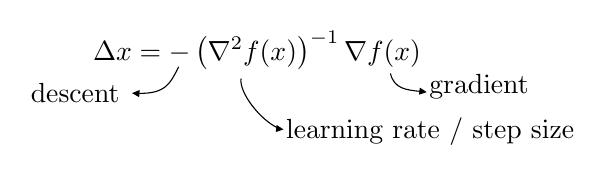
\begin{tikzpicture}[x=0.75pt,y=0.75pt,yscale=-1,xscale=1]
            %uncomment if require: \path (0,85); %set diagram left start at 0, and has height of 85
            
            %Curve Lines [id:da9054355359283472] 
            \draw    (262.66,40.29) .. controls (275.79,40.45) and (277.82,35.56) .. (282,27.5) ;
            \draw [shift={(259.5,40.17)}, rotate = 3.58] [fill={rgb, 255:red, 0; green, 0; blue, 0 }  ][line width=0.08]  [draw opacity=0] (3.57,-1.72) -- (0,0) -- (3.57,1.72) -- cycle    ;
            %Curve Lines [id:da9392696379295649] 
            \draw    (329.55,56.79) .. controls (321.59,53.21) and (311.12,40.25) .. (312,33.17) ;
            \draw [shift={(332.5,57.67)}, rotate = 187.13] [fill={rgb, 255:red, 0; green, 0; blue, 0 }  ][line width=0.08]  [draw opacity=0] (3.57,-1.72) -- (0,0) -- (3.57,1.72) -- cycle    ;
            %Curve Lines [id:da3170526273403007] 
            \draw    (398.42,39.33) .. controls (391.64,38.65) and (385.74,38.07) .. (384,30.67) ;
            \draw [shift={(401.5,39.67)}, rotate = 187.13] [fill={rgb, 255:red, 0; green, 0; blue, 0 }  ][line width=0.08]  [draw opacity=0] (3.57,-1.72) -- (0,0) -- (3.57,1.72) -- cycle    ;
            
            % Text Node
            \draw (239.5,8.9) node [anchor=north west][inner sep=0.75pt]    {$\Delta x=-\left( \nabla ^{2} f( x)\right)^{-1} \nabla f( x)$};
            % Text Node
            \draw (209.5,34) node [anchor=north west][inner sep=0.75pt]   [align=left] {descent};
            % Text Node
            \draw (332.5,51) node [anchor=north west][inner sep=0.75pt]   [align=left] {learning rate / step size};
            % Text Node
            \draw (401.5,30) node [anchor=north west][inner sep=0.75pt]   [align=left] {gradient};
            
        \end{tikzpicture}

        \begin{itemize}
            \item $\nabla^2 f \succ 0 \Rightarrow$ descent (minima).
            \item $\nabla^2 f \prec 0 \Rightarrow$ ascent (maxima).
        \end{itemize}
        \item In $\mathbb R^n, \nabla^2f\succ0, \nabla^2f\in S_{++}^n$, i.e. positive definite, $\Rightarrow \text{descent}$. In this case, we also call $f(x)$ ``strong convex''. These optimization problem can always be solved by Newton's method.
        \item However, the hessian matrix is not positive definite for most hard / nonlinear problems in robotics and other control systems. How to deal with them? We always can do some tricks --- regularization.
    \end{itemize}
    \item Regularization (Damped Newton's Method)
    \begin{itemize}
        \item Practical solution to make sure we're always minimizing.
        
        \begin{algorithmic}[1]
            \STATE $H\leftarrow\nabla^2f$
            \WHILE {$H\nsucc 0$} 
              \STATE $H\leftarrow H+\beta I, \quad \beta$ is a positive scalar hyper parameter
              \STATE Ant other idea? Flip or clip the eigen values?
            \ENDWHILE
            \STATE $\Delta x = -H^{-1}\Delta f$
            \STATE $x\leftarrow x+\Delta x$
        \end{algorithmic}

        \item Also called ``Damped Newton'' or ``Tikhonov regularization'' or ``quadratic pendalty'' or ``L2 loss''. Why ``damping''? Integrate the line 3, we add something related to $x$ to cost function, it's equivalent to having a $\beta \Delta x^T\Delta x$ added to the cost function, which shrinks (penalizes) step length $\Delta x$, but guarantees descent. It slows down the convergence, so don't use it unless needed. This method is similar to L1(lasso) and L2(ridge) regulation in machine learning. (For more information, search Google for \textbf{Tikhonov regularization} and \textbf{Levenberg-Marquarelt}).
    \end{itemize}
    \item Example:
    \begin{figure}[H]
        \centering
        
\includegraphics[scale=.75]{./tex/ch3/5.pdf}
        \caption{Minimization Starting From $x=0.0$ (w/ regularization, find local minima)}
    \end{figure}
    
    Now we can always find local minima.

    \item But what about overshooting?  This will cause the problem to diverge and never make it to the answer. We'll introduce line search method to solve this problem.
\end{itemize}
\subsection{Line Searching}
\begin{itemize}
    \item Often $\Delta x$ step from Newton overshoot the minima. To fix this, check $f(x+\Delta x)$ and ``back track'' until we get a good reduction. (similar to learning rate decay).
    \item There is another way called trust region besides line search.
    \item A simple effective one is \textcolor{red}{``Armijo rule''}.
    \begin{algorithmic}[1]
        \STATE $\alpha=1$ (initial step length)
        \WHILE {$f(x+\alpha x) > f(x) + b\alpha\nabla f^T(x) \Delta x$}
          \STATE $\alpha\leftarrow c\alpha, c\in(0,1)$
        \ENDWHILE
    \end{algorithmic}
    Making sure linearization step stay in tolerance $b$ of first-order Taylor expansion. Typically, $c=0.5,b=10^{-4}\sim0.1$. (any non-zero $b$ works)

    When $\alpha \to 0$, $f(x+\alpha x) = f(x) + \alpha\nabla f^T(x) \Delta x$.
    \item There is a second order version of these things called ``The Wolf conditions'' that use the Hessian, so those might be more Newton flavored and that they use also use the second order term in the Taylor expansion.
    \item At the the end of the day, I use a Taylor expansion to compute $\Delta x$ and use that Taylor expansion I predict some decrease in $f$, if that prediction from the Taylor expansion disagrees with what the actual function says then I stepped too far for the Taylor expansion to be valid such that third and fourth order terms in the Taylor expansion started to dominate then this would be bad.
    \item Both line search and trust region are saying can I trust the Taylor expansion.
    \item Example:
    \begin{figure}[H]
        \centering
        
\includegraphics[scale=.75]{./tex/ch4/1.pdf}
        \caption{Minimization Starting From $x=0.0$ (w/ regularization and line searching, find local minima, no overshooting)}
    \end{figure}
    \item Newton with simple, cheap modifications (globalization strategies) is extremely effective at finding local optimum. Since such strategies make each step out of the so-called ``epsilon ball'', they are ``global'', which means it's guaranteed to converge to a local Optimum globally from anywhere you start.
    \item However, in these cases when modifications is required, the Newton is no longer quadratic convergence.
\end{itemize}
\section{Supplement 2}

\subsection{Newton's Method}

\begin{itemize}
    \item Newton's method: a way to find root. A root is the solution to the equation $r(x) = 0$. P.S. anything we want to turn into $0$ is called \textbf{residual}.
    \item This is an example of a set of equations that would be basically impossible to solve by hand:
    \begin{equation}
        \begin{bmatrix}
        x_{1}^{2}\tan x_{3}^{\cos x_{2}}\\
        \sin x_{3}^{4} +e^{x_{1}}
        \end{bmatrix} =\begin{bmatrix}
        0\\
        0
        \end{bmatrix}
    \end{equation}
    \item This on the other hand is linear, we have 2 equations and 2 unknowns and can just solve for with substitution:
    \begin{equation}
        \begin{bmatrix}
        ax_1+bx_2\\
        x_2-3x_1
        \end{bmatrix} =\begin{bmatrix}
        0\\
        0
        \end{bmatrix}
    \end{equation}
    \item The point being made here is that we can't solve any $r(x) = 0$, but we can if it's linear, so what do we do? We take a first order Taylor series of $r(x)$ about some current value $x_k$ (giving us a linear approximation of $r(x)$), and solve that for when that is $0$:
    \begin{equation}
        r( x) =r( x_{k}) +\left. \frac{\partial r}{\partial x}\right| _{x_{k}}( x-x_{k}) =0\Rightarrow x=x_{k} -\left. \frac{\partial r}{\partial x}\right| _{x_{k}}^{-1} r( x_{k}) \Rightarrow x_{k+1}
    \end{equation}
    Here we take the Taylor expansion and solve for when that equals 0, and set that new value to be $x_{k+1}$.
    \item Now I can rewrite the Taylor series using delta notation, and just solve for the $\Delta x$ (this is identical to above):
    \begin{equation}
        r( x_{k} +\Delta x) =r( x_{k}) +\left. \frac{\partial r}{\partial x}\right| _{x_{k}} \Delta x=0\Rightarrow \Delta x=-\left. \frac{\partial r}{\partial x}\right| _{x_{k}}^{-1} r( x_{k})
    \end{equation}
    In this case, we can make it more flexible: $x_{k+1} = x_k + \alpha \Delta x$, in which $\alpha$ is called step size or learning rate.
    \item Newton's method has ``quadratic convergence'' meaning the error gets squared at every iterate $e_{k+1} = e_k^2$. This only happens once you are in the ``basin of attraction'' (small neighborhood), it is a local method.
\end{itemize}
\subsection{Optimization}
In general, the goal of optimization is to find the minima of function $f(x)$. For an unconstrained optimization problem, we have an optimality condition that says the gradient of the objective function w.r.t. $x$ must be $0$. This is just another root-finding problem where the ``residual function'' before is just the gradient of $f$. We can solve this by just doing normal Newton. The Jacobian of the gradient of $f(x)$ is the hessian of $f(x)$. The Newton step is computed as the following:

\begin{equation}
    \nabla _{x} f( x) =0\Rightarrow r( x) =\nabla _{x} f( x) =0\Rightarrow \Delta x=-\left(\left. \frac{\partial \nabla _{x} f( x)}{\partial x}\right| _{x_{k}}\right)^{-1} \nabla _{x} f( x_{k}) =-\nabla _{x}^{2} f( x_{k})^{-1} \nabla _{x} f( x_{k})
\end{equation}

This is why people talk about how Newton is forming a ``quadratic approximation'' of the cost function and minimizing that. Here is that ``quadratic approximation'' demonstrated.  If we take a second order Taylor series of $f(x)$ and minimize it, we get the equivalent Newton step:
\begin{equation}
    \min_{\Delta x} f( x_{k}) +( \nabla _{x} f( x_{k}))^{T} \Delta x+\frac{1}{2} \Delta x_{k}^{T} \nabla _{x}^{2} f( x_{k}) \Delta x\Rightarrow \Delta x=-\nabla _{x}^{2} f( x_{k})^{-1} \nabla _{x} f( x_{k})
\end{equation}

Now, let's take a brief look at KKT condition of a generic equality-constrained optimization problem where we don't assume anything about these functions.

\begin{equation}
    \begin{gathered}
        \min_{x} f( x) \quad x\text{: primal}\\
        \text{s.t.} \quad c( x) =0\quad \lambda \text{: dual}\\
        L( x,\lambda ) =f( x) +\lambda ^{T} c( x)\\
        \text{KKT conditions}\left[\begin{matrix}
        \nabla _{x} L=\nabla _{x} f( x) +\frac{\partial c}{\partial x}^{T} \lambda =0\\
        c( x) =0
        \end{matrix}\right. \\
        r\left(\begin{bmatrix}
        x\\
        \lambda 
        \end{bmatrix}\right) =\begin{bmatrix}
        \nabla _{x} L( x,\lambda )\\
        c( x)
        \end{bmatrix} =\begin{bmatrix}
        0\\
        0
        \end{bmatrix}
    \end{gathered}
\end{equation}
We can't just solve this anymore (since it's not linear in $x$ and $\lambda$) so we turn to our favorite method for rootfinding (Newton's method):

\begin{equation}
    \begin{bmatrix}
    \Delta x\\
    \Delta \lambda 
    \end{bmatrix} =\begin{bmatrix}
    \nabla _{x}^{2} L( x,\lambda ) & \frac{\partial c}{\partial x}^{T}\\
    \frac{\partial c}{\partial x} & 0
    \end{bmatrix}^{-1}\begin{bmatrix}
    -\nabla _{x} L( x_{k} ,\lambda _{k})\\
    -c( x_{k})
    \end{bmatrix}
\end{equation}

This is the so-called ``full'' newton. $\nabla _{x}^{2} L( x,\lambda ) = \nabla_x^2 f(x) + \frac{\partial}{\partial x}\left(\left(\frac{\partial c}{\partial x}\right)^T\lambda\right)$. The second term $\frac{\partial}{\partial x}\left(\left(\frac{\partial c}{\partial x}\right)^T\lambda\right)$ is the ``constraint curvature''. We often omit this term in practice. Because:
\begin{itemize}
    \item It can be very expensive to compute, we are differentiating a Jacobian wrt a vector, so we get a 3rd order tensor. 
    \item Usually in control we choose $f(x)$ so that it's nice and convex, making the hessian of $f(x)$ easy to compute and positive definite. This constraint curvature term can introduce negative eigenvalues into the hessian of the Lagrangian which makes Newton's method trickier to implement (since we would have to regularize to ensure a descent direction).
    \item $\nabla_x^2 f(x)$ in general is the dominant term and ``constraint curvature'' only adds a little bit and that's because the constraint non-linearity is not so insane that the second derivative of the constraints is is large enough to make a big difference and we also run the risk that it's expensive to compute. If constraint is linear, they are the same wether it is omitted.
\end{itemize}
Because of this, oftentimes in control we simply omit the constraint curvature term, and treat the hessian of the Lagrangian as if it were just the hessian of the cost function. This is called ``Gauss-Newton'', and it may take a little longer to converge depending on the scale of the problem. ``Gauss-Newton'':
\begin{equation}
    \begin{bmatrix}
    \Delta x\\
    \Delta \lambda 
    \end{bmatrix} =\begin{bmatrix}
    \nabla _{x}^{2} f( x ) & \frac{\partial c}{\partial x}^{T}\\
    \frac{\partial c}{\partial x} & 0
    \end{bmatrix}^{-1}\begin{bmatrix}
    -\nabla _{x} L( x_{k} ,\lambda _{k})\\
    -c( x_{k})
    \end{bmatrix}
\end{equation}
\subsection*{Least Square}
\begin{itemize}
    \item Prerequisite 1 - Quadratic form:
    \begin{equation}
        \begin{gathered}
            J( x) =\frac{1}{2} x^{T} Qx+q^{T} x\\
            \nabla _{x} J( x) =Qx+q\\
            \nabla _{x}^{2} J( x) =Q
        \end{gathered}
    \end{equation}
    We love this form of quadratic functions because we can take the derivatives of it really easily. We should always try and reduce things to this form when possible. \url{matrixcalculus.com} is a good website for playing around with these derivatives.
    \item Prerequisite 2 - Basic matrix manipulation:
    \begin{equation}
            \begin{gathered}
                ( ABC)^{T} =C^{T} B^{T} A^{T}\\
                x^{T} A^{T} b=b^{T} Ax\\
                ( Ax-b)^{T} =x^{T} A^T-b^{T}
            \end{gathered}
    \end{equation}
    These are 3 matrix manipulation tricks we will need to use in the following least squares examples.
    \item Least squares problems for ``skinny'' or overdetermined linear systems. This means there are more equations than there are unknowns, so we can't solve for $Ax=b$. Instead, we will solve for the $Ax \approx b$, and find the $x$ that gets us as close as possible. 
    
    \begin{equation}
        \begin{bmatrix}
        &  & \\
        &  & \\
        & A & \\
        &  & \\
        &  & 
        \end{bmatrix}\begin{bmatrix}
        \\
        x\\
        \\
        \end{bmatrix} \approx \begin{bmatrix}
        \\
        \\
        b\\
        \\
        \\
        \end{bmatrix}
    \end{equation}
    We rewrite the cost function and use our matrix manipulation tricks until we get our favorite quadratic form:
    \begin{equation}
            \begin{gathered}
                \begin{array}{ c l }
                \min_{x}\frac{1}{2}\Vert Ax-b\Vert _{2}^{2} & =\frac{1}{2}( Ax-b)^{T}( Ax-b)\\
                & =\frac{1}{2}\left( x^{T} A^{T} -b^{T}\right)( Ax-b)\\
                & =\frac{1}{2}\left( x^{T} A^{T} Ax-b^{T} Ax-x^{T} A^{T} b+b^{T} b\right)\\
                & =\frac{1}{2}\left( x^{T} A^{T} Ax-b^{T} Ax-b^{T} Ax\right)\\
                & =\frac{1}{2}\left( x^{T} A^{T} Ax-2\left( A^{T} b\right)^{T} x\right)\\
                & =\frac{1}{2} x^{T} Qx-q^{T} x
                \end{array}\\
                \nabla _{x} J( x) =A^{T} Ax-A^{T} b=0\Rightarrow x=\left( A^{T} A\right)^{-1} A^{T} b
            \end{gathered}
    \end{equation}
    $\left( A^{T} A\right)^{-1} A^{T}$ is the pseudo inverse for skinny $A$.
    \item Now let's look at ``fat'' or underdetermined linear systems where we have more variables than we do equations. This means we are able to satisfy $Ax=b$, but we want to find the $x$ with the smallest L2 norm that satisfies $Ax=b$:
    
    \begin{equation}
        \begin{bmatrix}
        &  &  &  & \\
        &  & A &  & \\
        &  &  &  & 
        \end{bmatrix}\begin{bmatrix}
        \\
        \\
        x\\
        \\
        \\
        \end{bmatrix} =\begin{bmatrix}
        \\
        b\\
        \\
        \end{bmatrix}
    \end{equation}
    This is an equality constrained optimization problem with a convex cost function and linear constraints. Form the Lagrangian and KKT conditions for optimality:
    \begin{equation}
        \begin{gathered}
            \min_{x}\frac{1}{2}\Vert x\Vert _{2}^{2}\\
            \text{s.t.} \quad Ax-b=0\\
            L( x,\lambda ) =\frac{1}{2} x^{T} x+\lambda ^{T}( Ax-b)\\
            \text{KKT condition:} \quad \begin{matrix}
            \nabla _{x} L( x,\lambda ) =x+A^{T} \lambda =0\\
            Ax-b=0
            \end{matrix} \Rightarrow x=A^{T}\left( AA^{T}\right)^{-1} b
        \end{gathered}
    \end{equation}
\end{itemize}
\section{Exercise 0}